% ==============================================================================
% frontmatter/cover.tex — หน้าปกนอก (3D Pixar Style - Transparent / No Background Box)
% ==============================================================================
\begin{titlepage}
\thispagestyle{empty}

\begingroup
\setlength{\XeTeXlinebreakskip}{0pt}

\begin{tikzpicture}[remember picture, overlay]
    % 1. ภาพอาร์ตเวิร์ก 3D Pixar แบบเต็มแผ่น (Full Bleed 6x9 in)
    \node[anchor=center, inner sep=0pt] at (current page.center) {
        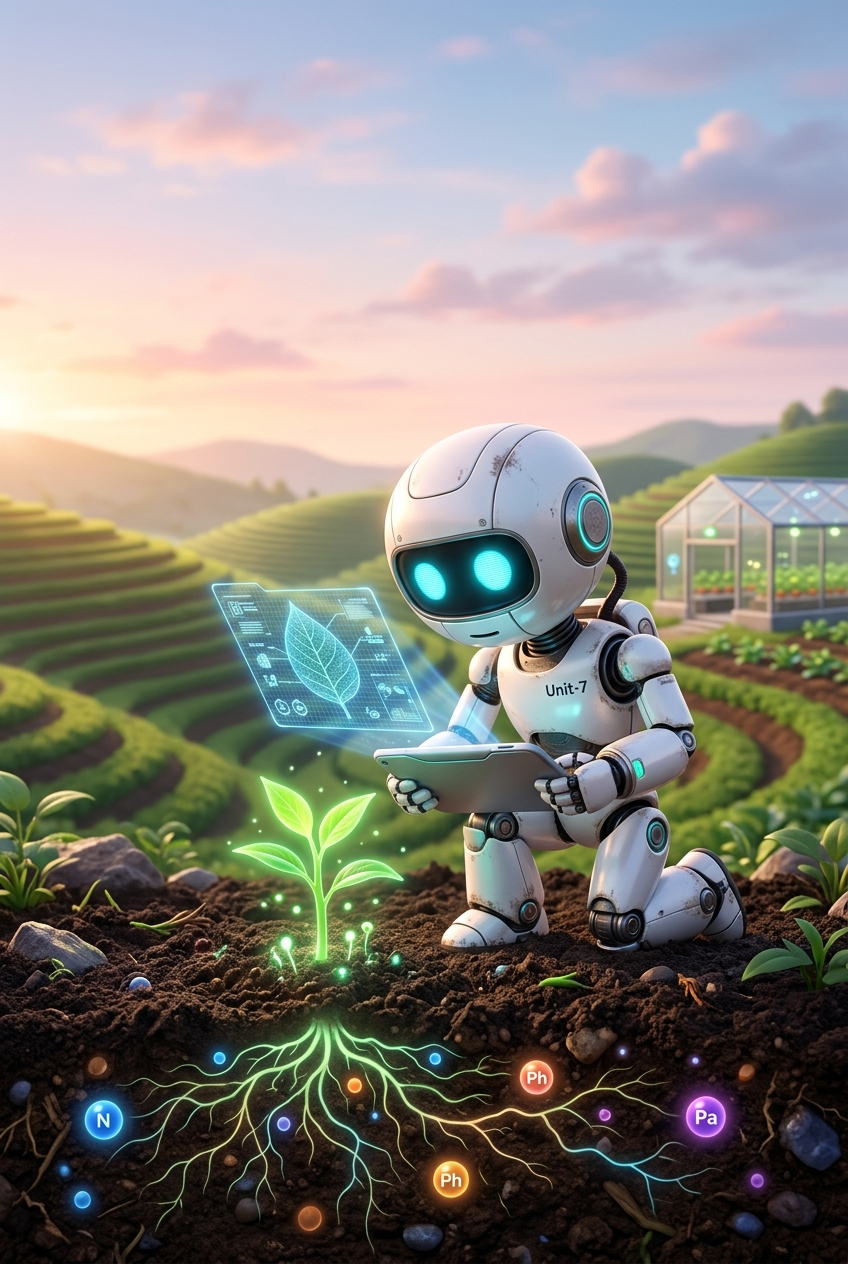
\includegraphics[width=\paperwidth,height=\paperheight]{figures/cover_art.jpg}
    };

    % 2. ข้อความชื่อเรื่องด้านบน (โปร่งใส ไม่มีกล่อง/พื้นหลัง พร้อมเงาเรืองแสงสีขาวเพื่อความคมชัด)
    % ชั้นเงาสีขาวบางๆ ช่วยให้อ่านง่ายบนท้องฟ้าธรรมชาติ (Shift 0.7pt)
    \node[anchor=north, align=center, text width=5.3in] at ([xshift=0.7pt, yshift=-0.41in]current page.north) {
        {\fontsize{8}{10.5}\selectfont\bfseries\color{white} HANDS-ON WORKSHOP HANDBOOK \textbullet\ เอกสารประกอบการอบรม}\\[6pt]
        {\fontsize{11}{14}\selectfont\bfseries\color{white} คู่มือการจัดเตรียมชุดข้อมูลและการฝึกอบรม}\\[4pt]
        {\fontsize{21.5}{26}\selectfont\bfseries\color{white} ปัญญาประดิษฐ์ฝังตัวและเอดจ์เอไอโอที\\[3pt]เพื่อการเกษตรและสิ่งแวดล้อม}\\[6pt]
        {\fontsize{8.5}{11}\selectfont\bfseries\color{white} EMBEDDED AI \& EDGE AIoT FOR AGRICULTURE AND ENVIRONMENT}\\[3pt]
        {\fontsize{7.5}{9.5}\selectfont\color{white} จากวิศวกรรมข้อมูลภาพระดับพิกเซลและเซนเซอร์เคมีดิน สู่การพัฒนาอุปกรณ์วินิจฉัยอัจฉริยะภาคสนาม}
    };
    % ชั้นตัวอักษรจริง (สีส้มสดใส และหลากสี สอดคล้องตามอัตลักษณ์เกษตรและสิ่งแวดล้อม)
    \node[anchor=north, align=center, text width=5.3in] at ([yshift=-0.42in]current page.north) {
        {\fontsize{8}{10.5}\selectfont\bfseries\color[HTML]{00695C} HANDS-ON WORKSHOP HANDBOOK \textbullet\ เอกสารประกอบการอบรม}\\[6pt]
        {\fontsize{11}{14}\selectfont\bfseries\color[HTML]{283593} คู่มือการจัดเตรียมชุดข้อมูลและการฝึกอบรม}\\[4pt]
        {\fontsize{21.5}{26}\selectfont\bfseries
            {\color[HTML]{E65100}ปัญญาประดิษฐ์ฝังตัว}{\color[HTML]{37474F}และ}{\color[HTML]{D84315}เอดจ์}{\color[HTML]{0277BD}เอไอโอที}\\[3pt]
            {\color[HTML]{2E7D32}เพื่อการเกษตร}{\color[HTML]{37474F}และ}{\color[HTML]{00838F}สิ่งแวดล้อม}
        }\\[6pt]
        {\fontsize{8.5}{11}\selectfont\bfseries\color[HTML]{263238} EMBEDDED AI \& EDGE AIoT FOR AGRICULTURE AND ENVIRONMENT}\\[3pt]
        {\fontsize{7.5}{9.5}\selectfont\color[HTML]{1565C0} จากวิศวกรรมข้อมูลภาพระดับพิกเซลและเซนเซอร์เคมีดิน สู่การพัฒนาอุปกรณ์วินิจฉัยอัจฉริยะภาคสนาม}
    };

    % 3. ข้อความข้อมูลผู้แต่งด้านล่าง (โปร่งใส ไม่มีกล่อง/พื้นหลัง วางที่ขอบล่างของผืนดิน)
    % ชั้นเงาดำช่วยขับให้อ่านชัดเจนแม้ทับซ้อนแนวแสง
    \node[anchor=south, align=center, text width=5.3in] at ([xshift=0.7pt, yshift=0.09in]current page.south) {
        {\fontsize{13.5}{17}\selectfont\bfseries\color{black} ผู้ช่วยศาสตราจารย์ ดร.ชีวะ ทัศนา}\\[2pt]
        {\fontsize{8.5}{11}\selectfont\color{black} สาขาวิชาปัญญาประดิษฐ์เพื่อเกษตรดิจิทัลและสิ่งแวดล้อม คณะวิทยาศาสตร์และเทคโนโลยี มหาวิทยาลัยราชภัฏรำไพพรรณี}\\[4pt]
        {\fontsize{8}{10}\selectfont\bfseries\color{black} โครงการพัฒนาผู้ประกอบการนวัตกรรมเกษตรและปัญญาประดิษฐ์ฝังตัว พ.ศ. 2569}
    };
    % ชั้นตัวอักษรจริงสีขาวสว่าง พร้อมไฮไลท์ทอง
    \node[anchor=south, align=center, text width=5.3in] at ([yshift=0.10in]current page.south) {
        {\fontsize{13.5}{17}\selectfont\bfseries\color{white} ผู้ช่วยศาสตราจารย์ ดร.ชีวะ ทัศนา}\\[2pt]
        {\fontsize{8.5}{11}\selectfont\color{white!95} สาขาวิชาปัญญาประดิษฐ์เพื่อเกษตรดิจิทัลและสิ่งแวดล้อม คณะวิทยาศาสตร์และเทคโนโลยี มหาวิทยาลัยราชภัฏรำไพพรรณี}\\[4pt]
        {\fontsize{8}{10}\selectfont\bfseries\color[HTML]{FFD54F} โครงการพัฒนาผู้ประกอบการนวัตกรรมเกษตรและปัญญาประดิษฐ์ฝังตัว พ.ศ. 2569}
    };
\end{tikzpicture}

\endgroup
\end{titlepage}
\cleardoublepage
